\documentclass{article}
    \usepackage[utf8]{inputenc}
    \usepackage[english]{babel}
    \usepackage[]{amsthm} %lets us use \begin{proof}
    \usepackage{amsmath}
    \usepackage{gensymb}   
    \usepackage{circuitikz} 
    \usepackage[margin=1in]{geometry}    
    \usepackage{mathrsfs}   
    \newcommand\underrel[2]{\mathrel{\mathop{#2}\limits_{#1}}}
    
\DeclareFontFamily{U}{calligra}{}
\DeclareFontShape{U}{calligra}{m}{n}{<->callig15}{}
\newcommand{\calE}{{\!\!\text{\usefont{U}{calligra}{m}{n}E}\,\,}}

    \usepackage[]{amssymb} %gives us the character \varnothing
    
    \title{PHY 316M}
    \author{Marc Matvienko}
    %This information doesn't actually show up on your document unless you use the maketitle command below
    
    \begin{document}
    \maketitle %This command prints the title based on information entered above
    \tableofcontents
    \section{Capacitors}
    $C = \lvert\frac{Q}{V}\rvert$

    \section{Current}
    Is the flow of charge in on direction.
    Current: $$I=\frac{\Delta Q}{\Delta t} =\frac{\delta Q}{\delta t}$$
    Current Density (current per unit area): $J = \frac{I}{A}$\\
    $n = \text{charge carriere density}$, $q = \text{charge per carrier}$, $v_d = \text{drift velocity}$
    This can give us, \boxed{$$J = nqv_d$$}
    
    \subsection{Ohm's Law}
    Usually we see Ohm's law in different forms, i.e. for a particular chunk.\\
    Consinder some block with volume $A \cdot l$, some source of energy(battery) forces current thorugh by applying an electric field.\\
    For a uniform electric field: \boxed{$$V = E\cdot l$$}
    
    \begin{align*}
        \begin{split}
            J &= \frac{I}{A} \\
            &= \sigma E \\
            &= \sigma \frac{V}{l}
        \end{split}
    \end{align*}
    $$\boxed{$$\frac{V}{I} = \frac{1}{\sigma} \frac{l}{A} = \rho \frac{l}{A} = R = \text{resistance}$$}$$
    \boxed{$$\frac{V}{I} = R$$}
    Resistance is not resistivity (opisiton of current flow of a particular material[$\rho$])
    Ohmic material is a material that has a constant slope on Voltage to Current graph. Most common materials like copper behave like this.
    %Section and subsection automatically number unless you put the asterisk next to them.
    \paragraph{Example} The resistivity of nichrome wire( heaters, toasters) is $1.5 \times 10^{-6}\Omega m$. 
    If a household voltage of $115V$ is applied acros a $0.2mm$ radius write, $1.0m$ long, what current flows?
    \paragraph{}$R = \rho \frac{l}{A} = \rho \frac{l}{\pi r^2} = \frac{1.5 \times 10^{-6}\Omega m \cdot 1.0 m}{(\pi (2\times 10^{-4}m)^2))} = 11.9 \Omega$    
   
    \subsection{Model for electric conduction}
    \begin{itemize}
        \item electron unergo many rapid ocllision when  $E = 0$
        \item when $E \neq 0$, the electrons accelrate between collisions
        \item $F = ma = qE => a = \frac{qE}{m}$
        \item $v = v_0 + at= v_0 + \frac{qE}{m}t $
    \end{itemize}
    Let $\tau = \text{average collision time} = R\cdot C$\\
    the  $v_d = v_{avg} = <v_0> + \frac{qE}{m}\tau$\\
    so, $J = nqv_d = nq = \frac{qE}{m}\tau = \sigma E$\\
    so conducitvity $\sigma = \frac{nq^2\tau}{m}$\\
    Called the Drude model or free electron mode\\
    $$\boxed{$$\sigma = \frac{nq^2 \tau}{m}$$}$$
    $$\boxed{$$\frac{1}{\sigma} = \rho$$}$$
    \paragraph{Example} Assume for copper that each atom donates one free electron. What is the average time between collision for electrons in copper.?
    \\Given: 
    \begin{itemize}
        \item Density$ = 8.98\frac{g}{cm^3}$
        \item Atomic Weight $ = 63.54\frac{g}{mole}$
        \item $\rho = 1.7 \times 10-^{-8}\Omega\cdot m$
    \end{itemize}
    $\tau = \frac{m}{nq^2\rho}=\frac{9.14 \times 10^{-31}kg}{(8.5\times10^22 ) (1.6\times10^{-19})^2 1.7\times10^{-8}\Omega m} = 2.5\times10^{-14}s$
    \subsection{Temperature Dependence of resistivity}
    \begin{itemize}
        \item resistivities tabulated for 20 \degree celsius
        \item for metals, $\rho$ is higher and T is higher
        \item $\alpha = \text{linear temprature coefficient}$
        \item over some range, \boxed{$$\rho = \rho_0 (1+ \alpha(T-T_0))$$}
    \end{itemize}
    As T increases, the scattering time decreases due to collisions with vibrating atoms\\
    At higher temperatures the $\rho$ to temprature graph  is linear. But at the beginning there is residual resistvity due to impurities.
   \paragraph{Semiconductors} The number of carriers decreases as the temperature decreases, this means that all the electrons are sticking to their atoms.
   \section{Resistors}
    Circuit symbol: 
    \begin{circuitikz}\draw
        (0,0)to[resistor, l=$R$] (4,0)
    ;\end{circuitikz}
    \subsection{Resistors in series} For resistors in series the resistivities add
    $$R_{tot} = R_1 + R_2 + ...$$
    $$R_{tot} = \frac{V}{I} = \frac{V_1}{I_1} + \frac{V_2}{I_2} = R_1 + R_2$$ 
    The current ( I ) is the same everywhere too.\textbf{ Resistors don't add in parallel. Capacitors do.}
    $$V = V_1 + V_2$$ 
    \\The voltage divider $$V_1 = I\cdot R_1 = \frac{V}{R_1 + R_2}\cdot R_1$$
    \subsection{Resistors in parallel}
    For resisitors in parallel halve the resistance if two exact resistors are put in parallel    
    \begin{itemize}
        \item In parallel have the same voltage across each element
        \item In parallel also the current divides among branches
    \end{itemize}
    $$I = I_1 + I_2 = \frac{V}{R_1} + \frac{V}{R_2} => R_{tot} = \frac{V}{I} = \frac{1}{\frac{1}{R_1}+\frac{1}{R_2}}$$
    \paragraph{Superconductors} Electrons pair up and when electron jumps to the lattice another electrons pulls it right back.
    \subsection{Resistors Disipate Energy}
    Electrons undergo collisions, and give up energy as heat. A steady release of current ($I$) causes a steady realease of energy.
    $$\Delta U = \Delta QV$$
    Better to discess the rate, which is really known as:
    $$\text{Power}=P=\frac{\Delta U}{\Delta t} = \frac{\Delta U}{\Delta t} V = IV$$
    $$\boxed{$$P = IV = I^2R = \frac{V^2}{R}$$}$$
    This power is also known as Joule heating.
    \paragraph{Putting this into practice:}many circuits can be analyzed with just Ohm's Law and Resistance.
    \begin{itemize}
        \item What is the total power delivered? 
        \item What is the power dissipated in each R?
    \end{itemize}
    \begin{circuitikz}\draw
        (0,-2)to[battery, l=$12V$] (0,1)
        (0,1) to (3,1)
        (3,1)to[resistor, l=$2\Omega$](3,-1)
        (2, -1)to(4,-1)
        (2,-1)to[resistor, l=$3\Omega$](2,-3)
        (4,-1)to[resistor, l=$6\Omega$](4,-3)
        (2,-3)to(4,-3)
        (3,-3)to(3,-4)
        (3,-4)to(0,-4)
        (0,-4)to(0,-2)
    ;\end{circuitikz}
    $P_{\text{dissapated in } 3\Omega} = \frac{V_3^2}{R} = \frac{(6V)^2}{3\Omega}=12W$
    \subsection{Direct Current Circuits}
    Real battery is an ideal $\calE$MF plus intended resistance\\
    \begin{circuitikz}\draw
        (0,0)
        node[label={left:Batteries are a source of voltage}] {}
        to[battery, l=$+$](2,0)
    ;\end{circuitikz}
    \\Source of voltage = "electromotive force" = $\calE$MF= $\calE$
    $$\boxed{$$V = \calE - Ir$$}$$
    "Open-circuit voltage", where $I=0$
    
    \paragraph{Analysis of circuits}
    Any circuit can be analyzed with Kirchhoffs Rules:
    \begin{itemize}
        \item Junction Rule, algebraic sum of currents into a junction = sum of currents $\Sigma i_{in} = \Sigma i_{out}$
        \item Loop Rule, algebraic sum of voltages around any closed loop is zero. Where voltage rises are positive (- to +) and votlage drops are negative (+ to -)
    \end{itemize}
    For resistors the current directino determines voltage drop(negative)

    \paragraph{Example}
    \begin{itemize}
        \item What is the current in the $6 \Omega$ resisitor?
        \item Is it flowing up or down?
    \end{itemize}
    \begin{circuitikz}\draw
        (0,-2)to[battery,l=$12V$](0,2)
        (0,2)to[resistor, l=$4\Omega$](4,2)
        (4,2)to[resistor, l=$6\Omega$](4,-2)
        (4,2)to[resistor, l=$2\Omega$](8,2)
        (8,2)to[battery,l=$12V$](8,-2)
        (0,-2)to(8,-2)
    ;\end{circuitikz}\\
    \begin{itemize}
        \item [\textbf{(I)}]Junction at A: $i_1 = i_2 + i_3$
        \item [\textbf{(II)}] Loop A: $12V - i_1(4\Omega) - i_3(6 \Omega) = 0$
        \item [\textbf{(III)}]Loop B: $I_3(6\Omega) - i_2(2\Omega) + 12V = 0$
    \end{itemize}
 
    $i_3 = \frac{-12V}{22\Omega} = -\frac{6}{11}A$
    \paragraph{2 other techniques:}
    \begin{itemize}
        \item[i)] same, except use ficticious ``loop currents''
        \item[ii)] Source suppressing - can look at effects of sources seperately
    \end{itemize}
    \paragraph{Next: Circuits with Capacitors} will see time-depedent behavior
    Before ``transient phenomena'', look at \textit{Steady-state}: ``after a long time''. The capacitor starts acting like the current is 0.

    \section{Magnetism}
    We saw: $$F = qv\frac{\mu_0 I}{2\pi r} = 0$$
    for $\vec{v}$ tangent to circle.
    where $\mu_0 = 4\pi \times 10^{-7} \frac{Ns^2}{C^2}$\\
    Rewrite this as $$\boxed{$$\vec{F} = q\vec{v}\times \vec{B}$$}$$
    where \boxed{$$B = \frac{\mu_0 I}{2 \pi r}$$} magentic field due to a long wire where direciton of $\vec{B}$ is tangent to circle.
    \\If also electric force, combination of electric and magnetic force is called ``Lorentz Force'' $$\vec{F} = q\vec{E} + q\vec{v}\times \vec{B}$$
    $\vec{F} = q\vec{v}\times \vec{B}$
    \begin{itemize}
        \item Like $\vec{E}, \vec{F}$ opposite for $+q, -q$
        \item Depends on $\vec{v}: \vec{F} = 0 \text{ for } \vec{v} = 0$
        \item Depends on angle : \boxed{$$\lvert\vec{F}\rvert = \lvert q \rvert v B sin\Theta$$}\\
        notice $\vec{F} = 0$ for $\vec{v} \parallel \vec{B}$
        \item Direction $\vec{F} = q\vec{v}\times\vec{B}$ given by right hand rule
    \end{itemize}
    Magnetic field does no work because the magnetic force is perpendcular to displacement.\\
    So $\vec{B}$ changes direction of $\vec{v}$ but not its magnitude ($KE = \frac{1}{2}mv^2$)\\
    Unit of B = $\frac{Ns}{Cm} = \text{tesla} = T$ also gauss $= G = 10^{-4} T$
    \subsection{Evaluating Cross Products}
    \begin{itemize}
        \item [1.] Get general equation by expaning determinant 
        $\begin{vmatrix} i & j & k \\ v_x & v_y & v_z \\ B_x & B_y & B_z\end{vmatrix} = $\\
            $\vec{v}\times \vec{B} = i(v_yB_z-v_zB_y) - j(v_xB_z - v_zB_x) + k(v_xB_y-v_yB_x)$
        \item [2.] Just multiply out.\\
        know that $i \times j = k$ and that $j \times i = -k$
        \item [5.] Magnetic field does no work
    \end{itemize}
    \subsection{Ampere's and Biot Savart Law}
    \begin{enumerate}
        \item Ampere's Law: for high symmetry
        \item Biot Savart Law
    \end{enumerate}
    In general we will only look at: center of arcs and circles, or due to straight segments, or on axis of loop.
    \subsubsection{$\vec{B}$ at the center of a circle}
    $$d\vec{B} = \frac{\mu_0}{4\pi}\frac{Id\vec{s}\times \hat{r}}{r^2}$$
    $$B = \int dB = \int \frac{\mu_0 I}{4 \pi r^2}ds = \frac{\mu_0 I}{2R}$$
    Since $r=R$, the integral is constant and is easy to integrate with respect to s.
    \paragraph{Also:}for a fraction f of a circle \boxed{$$\vec{B} = fB_{\text{full circle}}$$}
    
    \subsubsection{$\vec{B}$ near a finite straight wire}
   
    \begin{align*}
        \begin{split}
            d\vec{B} &= \frac{\mu_0 I}{4\pi}\frac{d\vec{s}\times \hat{r}}{r^2}\\
                &= \frac{\mu_0 I}{4\pi} \frac{ds sin\theta}{r^2}
        \end{split}
    \end{align*}

    \begin{enumerate}
        \item $sin\theta = sin\theta ' =cos\phi$
        \item $cos\phi = \frac{R}{r} \rightarrow r \frac{R}{cos\phi}$
        \item $tan\phi = \frac{s}{R} \rightarrow s =R\cdot tan\phi \rightarrow \frac{R}{cos^2\phi d\phi}$
    \end{enumerate}

    \begin{align*}
        \begin{split}
            B &= \int dB \\
            &= \int \frac{\mu_0I \frac{R}{cos^2\phi}d\phi cos\phi}{4\pi (\frac{R}{cos\phi})^2} \\
            &= \frac{\mu_0 I}{4\pi R}\int_{-\phi_1}^{+\phi^2}cos\phi d\phi \\
            &= \frac{\mu_0 I}{4\pi R}sin \phi \rvert_{-\phi_1}^{+\phi^2} \\
            &= \frac{\mu_0 I}{4\pi R}[sin \phi _2 + sin\phi _1]
        \end{split}
    \end{align*}

    \subsubsection{B field due to a square loop of side a}
    $$B_{loop}$$
    $$\frac{2\sqrt{2}\mu_0 I}{\pi a}$$

    \subsubsection{B on axis of loop}
    Off axis compnents cancel around circle. \\
    $\phi$ is the angle at the bottom right of triangle formed by circle and axis
    \begin{align*}
            r &= \sqrt{x^2 + R^2} && \text{Using pythagorean theorem}\\
            sin\phi &= \frac{R}{\sqrt{x^2 +R^2}} && \text{So we can define }sin\phi
    \end{align*}
    We only have to integrate along the x compnents
    \begin{align*}
            dB_x &=dB sin\phi \\
            &= \frac{\mu_0 I ds}{4\pi r^2}sin\phi
    \end{align*}
    We can say that $\int \,ds = 2\pi R $ since the radius is constant\\
    \begin{align*} 
        B &= \int \frac{\mu_0 I}{4\pi r^2}sin\phi \,ds\\
        &= \frac{\mu_0 I R}{4 \pi (x^2+R^2)^{3/2}}\int \,ds\\
        &= \frac{\mu_0 I R^2}{2 (x^2+R^2)^{3/2}}     
    \end{align*}
    
    Also, consider yourself very close to the field, $ x >> R ~ \frac{1}{x^3}$ dipole field
    \subsection{Motion in a uniform $\vec{B}$}
    $$ \lvert \vec{F} \rvert = \lvert q\vec{v} \times \vec{B} \rvert = qvB $$
    $\vec{F}$ is $\bot$ to $\vec{v}$ centripetal with accelarations $a_r = \frac{v^2}{r}$
    We saw that 
    \begin{align*}
        B_{\text{long wire}} &= \frac{\mu_0 I}{2\pi r}\\
        B_{\text{solonoid}} &= \mu_0 n I \\
        B_{\text{loop center}} &= \frac{\mu_0 I}{2R}
    \end{align*}
    $\text{angular velocity } \omega = ?$
    $$r = \frac{mv}{qB}$$
    \paragraph{Example: Mass Spectrometer}
    \textit{Note: Electrons travel in a semi-circle in a spectrometer}
    Electrons are accelarated through potential of $10^3 V$ ("a 1 keV electron"). 
    They enter a region of uniform $B = 10^{-2}T$. What is the distance they are displaced?
    $$x = 2r = 2 \frac{mv}{qB}$$\\
    Know $m,q,B$ need to find $v$\\
    \begin{align*}
        \Delta KE &= \Delta PE \rightarrow \frac{1}{2}mv^2 = eV_0= \sqrt{\frac{2eV}{m}} \\
        x &= 2\frac{m}{eB}\sqrt{\frac{2eV_0}{m}} = \frac{2}{B}\sqrt{\frac{2mV_0}{e}} = \frac{2}{(10^{-2}T)}\sqrt{\frac{2(9.11\times 10^{-31})(10^3V)}{(1.6\times 10^{-19}C)}}        
    \end{align*}
    \\In practice however, we are given v,B,x to get ($\frac{q}{m}$)

    \paragraph{Example: Velocity Selector}region of crossed $\vec{E} + \vec{B}$\\
    All we have to consider is $qE \textit{ -vs- } qvB$\\
    if $qE = qvB$ then \boxed{$$v = \frac{E}{B}$$}

    \subsection{Force on a current}
    Consider positive charge travelling along x axis with $v_0$ with a $-\vec{B}\hat{y}$
    \begin{align*}
        F_{\text{on wire}} &= q\vec{v}\times\vec{B}\\
        &= \frac{1}{n}\vec{j}\times\vec{B}\\
       F_{\text{on wire}}&=\text{(\# charges)}F_{\text{on 1 charge}}\\
       &=(nAl)\frac{1}{n}\hat{\vec{j}}\times\hat{\vec{B}}\\
       &=lA\vec{j}\times\vec{B}\\
       &=I\vec{l}\times\vec{B}
    \end{align*}
    \paragraph{Example}
    Net force on a current loop in a uniform $\vec{B}$ is \textbf{zero}. 
    This is true for any loop.
    \paragraph{Example} A current I flows from the origin to $(x,y,z) = (1m,1m,0)$ and then straight to $(2m,0,0)$. In a uniform field of $\vec{B} = 5T\hat{i}$
    \begin{align*}
        \vec{F}_1 &= (10N)(-\hat{j} + \hat{i})\\
        \vec{F}_2 &= (10N)(-\hat{j}-\hat{i})\\
        \vec{F} &= (20N)-\hat{j}
    \end{align*}

    \paragraph{Example} Force on a wire segment due to a large $\parallel$ wire
    \begin{align*}
        B &= \frac{\mu_0 I}{2\pi r}\\
        \vec{F} &= I_2\vec{l}\times \frac{\mu_0 I_1}{2\pi r}\\
        &= I_2\times \frac{l \mu_0 I_1}{2\pi r}\\
        \frac{\text{force}}{\text{length}} &= \frac{\mu_0 I_1 I_2}{2\pi r}
    \end{align*}
    \paragraph{Definition:}Magnetic Moment\\
    Dipole moment ($\mu = IA$) due to a magnetic loop.
    \subsection{Torque on a current}
    \paragraph{We saw:} $\vec{F} = I\vec{l}\times \vec{B}$
    \paragraph{Magnetic Moment} $\vec{\mu} = I\vec{A}$\\
    and for N loops we have $\vec{\mu} = NI\vec{A}$
    \paragraph{we also saw that}for a loop in uniform $B \rightarrow \vec{F} = 0$. 
    There is no force, but there is a \textbf{net torque}.
    \paragraph{Torque on a current\\Loop in a uniform B}

    \begin{align*}
        \vec{\tau} &= \Sigma\vec{r}\times\vec{F}\\
        \lvert \vec{\tau}\rvert &= \Sigma rFsin\theta\\
        &= (z)(\frac{l}{z})I l B sin \theta \\
        &= I l^2Bsin\theta \\
        &= \mu B sin\theta \\
        \vec{\tau} &= \vec{\mu} \times \vec{B}
    \end{align*}
    Where $\mu$ is the magnetic moment and $\vec{B}$ is the magnetic field.
    \section{Magnetism and Matter}
    \paragraph{} Comes from some sort of current loop in matter. Perhaps an electron traveling around a proton, that is a current loop. 
    \paragraph{Example} Consider the oribting elctron as current:
    $$I = \frac{\Delta Q}{\Delta t} = \frac{e}{T} = \frac{e}{(2\pi r) / v} = \frac{e\cdot v}{2\pi r}$$
    $$\mu = IA = \frac{e\cdot v}{2\pi r} \cdot \pi r^2 = \frac{1}{2}evr$$
    Recall that angular momentum is $\vec{l} = \vec{r} \times \vec{p}$ and therefore \boxed{$$l=mvr$$}
    $$\mu = \frac{e}{2m}mvr = \frac{e}{2m}l$$
    \\An atom can have many electrons $\vec{L} = \Sigma \vec{l_i}$ and that $\mu = -\frac{e}{2m}\vec{L}$
    \subsection{Quantum Mechanics} $\vec{l}$ is quantized: $l = 0, \hbar, 2\hbar, ...$ 
    When $\hbar = \frac{h}{2\pi} = 1.06\times 10^{-34}J$ where h = Planck's constant = $6.63\times 10^{-34}J$. 
    Ultimately, the spin of atom does not really exist, but it behaves like it is. Its ``spin'' would be $s = \frac{\hbar}{2}$
    $$\text{Adding total angular momentum } \vec{J} = \vec{L} + \vec{S}$$
    When $l = \hbar$ we have the smallest possible moment. $\mu = \frac{e\hbar}{2m} = \text{Bohr magneton} = 9.27\times 10^{-24}J/T$
    \subsection{Magnetization}
    \paragraph{Definition} Magnetization $ = M = \frac{\mu}{(volume)} = $ magnetic moment per unit volume. 
    \paragraph{The total field}In an external lfield, some moments align and they produce their own field, $\vec{B}_{matter}$.
    With our definitions, $B_{\text{matter}} = \mu_0 M$, so the total field $\vec{B} = \vec{B}_{ext} + \mu_0\vec{M}$. 
    For many field $\vec{B} \propto \vec{B}_{ext}$. 
    Really we can say that $\vec{B} = K_m \vec{B}_{ext}$ where $K_m = $ magnetic permeability or just the permeability constant.
    \paragraph{Vaccum} $K_m = 1$ 
    \paragraph{Diamagnet} in most materials $K_m - 1 \approx 10^{-6} - 10^{-4} \approx -10^{-5}$ because they have closed shells
    \paragraph{Ferromagnet} $K_m >> 1$ have locked moments due to Pauli exclusion principle. 
    \paragraph{Superconductors} Type I superconductors have a $K_m = 0$, which means they shield the cternal field.
    \paragraph{Magnetic Susceptibility} $\chi_m = K_m - 1$ \boxed{$$\frac{\mu_0M}{B_{ext}}$$}
    
    \subsection{Hall Effects}
    \subsubsection{Hall effect}is used for measuring the charge carrier dnesity $n$ (or, for known $n$, can measure B  or map B)
    \begin{description}
    \item Consider a current $I \text{ and a } \perp \vec{B}$
    \item Carrier experience $\vec{F} = q\vec{v} \times\vec{B}$, deflext and build up on surface with their transverse electric field balances magnetic force
    until $qE_t = qv_dB$
    \item We measure the (transverse) ``Hall Voltage'' $V_H = E_td$
    \item Use current density $j = \frac{I}{A} = \frac{I}{dl} = nqv_l \rightarrow v_d = \frac{I}{nqdl}$ (1)
    and $F_e = F_m \rightarrow E_t = v_dB \rightarrow v_d = \frac{E_t}{B}$ (2)
    \item Due to (1) and (2) we can say $\frac{E_t}{B} = \frac{I}{nqdl}$
    and $V_H = E_td \rightarrow \frac{V_H}{Bd} = \frac{I}{nqdl} \rightarrow$ \boxed{$$ n = \frac{IB}{V_Hql}$$}
    \end{description}
        
    \subsubsection{Motional EMF} 
    This gives us Magnetic Flux and Faraday's Law\\
    Instead of a current procing a Hall Voltage, we can just $\vec{v} \perp \vec{B}$. 
    Ions are stuck, but electrons can move, until $qE_t = qvB$ and get a transverse voltage.
    Called a \textbf{motional EMF}. \boxed{$$\calE = E_tl = Blv$$}. We will see many ways to get EMF by ``sweeping past B field''

    \section{Faraday's Law}
    Holds for any closed path, even the object producing the flux itself.
    \subsection{Preperation}
    $\calE = Blv$\\ Before looking at Faraday's Law define Magnetic Flux $\Phi _m = \int \vec{B}\cdot d\vec{A} = \vec{B}\vec{A} = BAcos\Theta$. We will be interested in ``flux through a current loop''.
    \paragraph{Example} A long solenoid with current $I$ and $n$ turns/meter, radius $R_2$ contains a loop of radius $R_1 \perp$ to solenoid axis. 
    Find flux through loop. Remember: \boxed{$$B_\text{solenoid} = \mu_0nI$$}.
    \\$$\Phi _m = \int \vec{B}\cdot d\vec{A} = \vec{B}\cdot \vec{A} = BA = (\mu_0 n I)(\pi R_1^2)$$
    Will only get an induced voltage if something is moving though.
    \paragraph{Example} A rectangular loop is ?? in plane of a long wire carrying current I. From wire to one end of rectangle is a, and to other end is b.
    \\Remember that B is not uniform. $$\Phi _m = \int \vec{B}\cdot d\vec{A} \underrel{\vec{B}\perp\vec{A}}{=} \int BdA 
    = \int_a^B \frac{\mu_0 I}{2\pi r} l dr= \frac{\mu_0 I l}{2\pi}\int_a^b \frac{1}{r} dr = \frac{\mu_0 I l}{2\pi} ln(b/a) $$

    \subsection{Content}
    A changing magnetic flux induces a current/voltage aroud a loop. 
    If $\Phi _m$ is the flux though surface then the voltage around that surface is 
    $$\calE = -\frac{\partial \Phi _m}{\partial t}$$
    If N loops on a coil then $$\calE = -N\frac{\partial \Phi _m}{\partial t}$$

    \paragraph{Example} A loop of wire with resistance R is partly in a region of uniform B and is pushed in at a constant $v$. What happens?
    
    \begin{description}
        \item $$\Phi = BA = Blx$$
        \item Faraday: $\calE =\frac{d\Phi}{dt} = -\frac{d}{d t}Blx = Bl \frac{dx}{dt} = -lv$. If loop is closed, current flows. $I = \frac{\calE}{R} = -\frac{Blv}{R}$. 
        \item Energy designated: $P = I^2R = \frac{B^2l^2v^2}{R}$. Another view: $\vec{F} = I\vec{l} \times \vec{B} = I;B = \frac{Blv}{R}lB$
        \item Hence we can say $P = Fv = \frac{B^2l^2v^2}{R}$
    \end{description}
    
    \paragraph{The sign in Faraday's Law} The ``-'' in the equation for $\calE$ is called 
    \textbf{Lenz' Law}, which states that induced current opposes the change in flux.
    \begin{description}
    \item We saw the EMF of a moving rod $\calE = Blv$
    \item Faraday's Law $\calE = -\frac{d\Phi}{dt}$, and Lenz' law tells us that the negative is there.
    \item $\Phi = \int \vec{B}d\vec{A} = BA cos\theta$
    \item $\calE = -\frac{d}{dt}(BAcos\theta) = Acos\theta \frac{dB}{dt}$    
    \end{description}
    \paragraph{Example} A rectabular loop with horizontal side of length 1m,
    loop resistance $0.1\Omega$, and a mass of $0.1kg$, is dropping out of 
    a region of uniform $B = 2T$. What is its terminal velocity?
    \begin{description}
    \item $F_{net} = 0 = F_g+F_m$
    \item We know induced voltage $\calE = Blv \rightarrow I = \frac{Blv}{R}$
    \item So $\lvert F_m \rvert = \lvert I\vec{L} \times \vec{B}\rvert = IlB = \frac{B^2l^2v}{R} \rightarrow \frac{B^2l^2v}{R} = mg$
    \item $v = \frac{mgR}{B^2l^2} = \frac{(0.1kg)(9.8m/s^2)(0.1\Omega)}{(2T)^2(1m)^2}$
    \end{description}
    \paragraph{Example}Two concentric loops with $R_1 = 1m$ and $R_2 = 1cm$. 
    Current in \#1 is increasing is increasing at $2A/s$. What is the Emf induced in loop \#2
    \begin{description}
        \item We know that $B_{\text{center of loop}} = \frac{\mu_0 I_1}{2R_1}$
        \item Then EMF $\calE = -\frac{d\Phi}{dt} =-\frac{d}{dt}BA = -\pi R_2^2\frac{dB}{dt}$
        \item or $\calE _2 = -\pi R^2_2\frac{d}{dt}\frac{\mu_0I_1}{2R_1} = -\frac{\pi R_2^2\mu_0 dI_1}{2R_1dt})$
        \item So we can get $\calE _2 = \frac{-\pi (0.01m)^2(4\pi\times10^{-7})}{2(1m)}(2A/s) = -4\times10^{-10}V = -400pV$
        \item Common situation: $\calE = -(\text{constant})\frac{dI_1}{dt}$
        \item We define $\calE_2 = -M_{12}\frac{dI_1}{dt}$
        \item Big / small loops = $M_{12} = \frac{\pi R_2^2\mu_0}{2R_1}$
    \end{description}
    \subsection{DC generator} Mechanical input creates electric output.
    Where $\theta = \omega t =$ rotations of the generator
    \begin{align*}
        \calE &= -\frac{d}{dt}BAcos\theta\\
        &= -BA \frac{d}{dt}cos\omega t\\
        &= \omega BAsin\omega t
    \end{align*}

    What is ``induced voltage around loop''? Even if no loop (no wire), to have voltage we must have an $\vec{E}$ field in space.
    \paragraph{Note} Different $\vec{E}$ arrangement than in electrostatics.
    \begin{description}
        \item Electrostatics: $V = \int \vec{E}\cdot d\vec{s}$, and also $\oint \vec{E}\cdot d\vec{s} = 0$
        \item But $\vec{E}$ fields due to changing $\vec{B}$, hence, $\calE = \oint \vec{E}\cdot d\vec{s} \neq 0$
        \item So we can have ``non-conservative'' fields
    \end{description}
    \paragraph{Note} Similarity beteween Ampere's Law and Faraday's Law 
    \paragraph{Ampere's}
    \begin{align*}
        \oint\vec{B}\cdot d\vec{s} &= \mu_0 I\\
        B(2\pi r) &= \mu_0 I \\
        B &= \frac{\mu_0 I}{2\pi r}
    \end{align*}
    \paragraph{Faraday's}
    \begin{align*}
        \calE = \oint\vec{E} \cdot d\vec{s} &= -\frac{d\Phi_m}{dt}\\
        E(2\pi r) &= \frac{d\Phi}{dt}\\
        E &= -\frac{-\frac{d\Phi}{dt}}{2\pi r}
    \end{align*}
    \begin{itemize}
        \item $r < R$ : $\Phi = \pi r^2 B \rightarrow E = \frac{r dB}{2 dt}$
        \item $r > R$ : $\Phi = \pi R^2B \rightarrow E = \frac{E^2 dB}{2r dt}$
    \end{itemize}
    \paragraph{Note} Electromagnetic safety suggests that one change B slowly to avoid a larg $\vec{E}$
    \paragraph{Example}Rotating rod in magnetic field. Held at one end and spins in magnetic field.
    Length l and spin of $\omega$. To get induced voltage do:
    \begin{align*}
        \calE &= -\frac{d}{dt}BA\\
        &= -B\frac{dA}{dt}\\
        &=-B\frac{\Delta A}{\Delta t}\\
        &= - B\frac{(\pi l^2)}{2\pi/\omega}\\
        &= -\frac{B\omega l^2}{2}
    \end{align*}
    \section{Inductance}
    For this recall, $\calE = -N\frac{d\Phi_M}{dt}$. This holds true for any closed path around $\Phi$.
    In particular, the changing current induces a voltage across the source itself.
    \begin{description}
        \item N is the number of turns
        \item $n = \frac{N}{l}$
        \item $B = \mu_0\frac{N}{l}I$
        \item So due to Faraday's law we can say that 
        \begin{align*}
            \calE &= -N\frac{d\Phi}{dt}\\
            &= -N\frac{d}{dt}(BA)\\
            &= -N\frac{d}{dt}(\mu_0\frac{N}{l}I)(A)\\
            &= -\frac{\mu_0N^2A}{l}\frac{dI}{dt}
        \end{align*}
    \end{description}
    \paragraph{Main feature}voltage indeed is proportianl to rate of change of current. 
    \\Constant of proportionality = L = ``self-inductance'' or  ``inductance''. \boxed{$$\calE = -L\frac{dI}{dt}$$}
    \\Similar, but opposite, to capacitance: $q=Cv$ or $\frac{dq}{dt} = C\frac{dV}{dt} = i$. 
    For magnetic fields $N\Phi \propto B \propto I_{\text{changing flux}}$.
    We can hence write, \boxed{$$N\Phi = LI$$}
    $\frac{d}{dt} \rightarrow -N\frac{d\Phi}{dt} = -L\frac{dI}{dt} \rightarrow$\boxed{$$v_L = -L\frac{dI}{dt}$$} this is also known as ``back emf''.
    Above for solenoid, \boxed{$$L = \frac{\mu_0 N^2}{l}A$$}. The unit of L is a henry, is in units of H $= \frac{V{-s}}{A}$.
    \paragraph{Note} If you fill coil with magnetic momtvial with permiability $K_m$ then $L = K_mL_0$.
    \\ Inductor symbols are: \\
    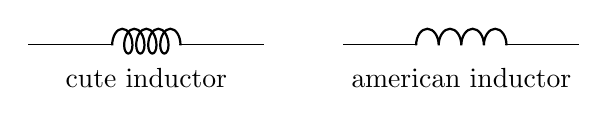
\begin{tikzpicture} 
        \draw (0,0) to[cute inductor] (3,0) ; 
        \node [below=5pt] at (1.5,0) {cute inductor};
    
        \draw (4,0) to[american inductor] (7,0) ; 
        \node [below=5pt] at (5.5,0) {american inductor};
    \end{tikzpicture}
    \subsection{RL circuits}
    \begin{enumerate}
        \item Steady state i.e. ``after a long time''. i is constant, $\frac{di}{dt}$\\
        \begin{circuitikz}\draw
            (-2,0)to[battery,l=$12V$](2,0)
            (2,0)to(2,2)
            (2,2)to[cute inductor](0,2)
            (0,2)to[resistor](-2,2)
            (-2,0)to(-2,2)
        ;\end{circuitikz}\\
        $v_L = -L\frac{di}{dt} = 0$
        \item Reponse to a sudden change in DC\\
        \begin{circuitikz}\draw
            (0,0)to[resistor](3,0)
            (0,0)to[battery](0,1)            
            (0,1)to[switch](3,1)
            (3,1)to[cute inductor](3,0)
        ;\end{circuitikz}\\
        \begin{align*}
            V_0 - L\frac{dI}{dt} - IR &= 0\\
            V_0 - IR &= L\frac{dI}{dt}\\
            I - \frac{V_0}{R} &= -\frac{L}{R}\frac{dI}{dt}\\
            \frac{dI}{I-V_0/R} &= -\frac{R}{L}dt\\
            \int_0^i\frac{dI}{I-V_0/R} &= -\frac{R}{L}\int^t_0dt\\
            ln[\frac{i-V_0/R}{-V_0/R}] &= -\frac{R}{L}t\\
            \frac{i-V_0/R}{-V_0/R} &= e^{-\frac{R}{L}t}
        \end{align*}
        So, 
        \begin{align*}
            v_L = -L\frac{dI}{dt} &= -L [\frac{d}{dt}(\frac{V_0}{R}(1-e^{-\frac{R}{L}t}))]\\
            &= -L\frac{V_0}{R}(e^{-\frac{R}{L}t})(-\frac{R}{L}) \\
            &= V_0e^{-\frac{R}{L}t}
        \end{align*}
        If we have switch in position 1 for a logn time $\frac{R}{L}t \rightarrow I = \frac{V_0}{R}$\\
        Switch to position 2 of $t=0$
    \subsubsection{Loop Theorem} $-L\frac{dI}{dt} - IR = 0$
        $$\int^{I_0}_I\frac{dI}{I} = -\int^t_0\frac{R}{L}dt \rightarrow ln(\frac{I}{I_0}) = -\frac{R}{L}t$$
    \end{enumerate}
    \subsection{Energy Stored Inductors}
    Power is $P = IV = \frac{dV}{dt}$, inductor $\frac{dV}{dt} = I (L\frac{dI}{dt})$,
    or $dI$ gives $dV$: $dV = LIdI$. 
    $V = \int dV = L \int^I_0IdI = LI^2\frac{1}{2}$
    Energy in inductor \boxed{$$V_L = \frac{1}{2}LI^2$$}
    \paragraph{Potential energy} One can think of this U as stored in B field
    \paragraph{Definition}magnetic energy per unit volume $$u_b = \frac{U_L}{\text{volume}} = \frac{1}{2\mu_0}B^2$$
    \section{Oscillators}
    Remember the formula for induction and L-R circuits
    Today we will discuss:
    \begin{enumerate}
        \item Free oscillations \textbf{LC, LRC}
        \item Forced oscillations \textbf{R, C , Power}
    \end{enumerate}
    \subsection{Natural/Free}
    \paragraph{}Combination of L and C is an oscillators
    \begin{itemize}
        \item First charge $C \text{ to } Q_0 = CV_0$
        \item Connect to $L$ at $t = 0$
    \end{itemize}
    Since we know
    $$I = -\frac{dQ}{dt}$$
    Loop: 
    \begin{align*}
        V_c-V_l &= 0 \\
        \frac{Q}{C} - L\frac{dI}{dt} &= 0 \\
        \frac{Q}{C} + L\frac{d}{dt}(\frac{dQ}{dt}) &= 0
    \end{align*}
    Ultimately, we get:
    $$\frac{d^2Q}{dt^2} + \frac{1}{LC}Q = 0$$
    \begin{enumerate}
        \item simplest 2nd order diff. eq.
        \item like simple harmonic oscillator, similar to solution of $Q = Acos(\omega t) + B sin (\omega t)$
    \end{enumerate}
    Only possible solutions $A + B$ are constant to be detemined by initial conditions and (like $\omega = \sqrt{\frac{k}{m}}$ for spring) here,
    \boxed{$$\omega = \frac{1}{\sqrt{LC}}$$} is the angular frequency of oscillator.
    We can check this by substituting:
    \begin{align*}
        \frac{d^Q}{dt^2} &= \frac{d^2}{dt^2}(Acos(\omega t) + B sin (\omega t))\\
        &= -\omega ^2[Acos(\omega t) + B sin (\omega t)]\\
        &= -\omega Q\\
        &= -\frac{1}{LC}Q\\
        \omega ^2 &= \frac{1}{LC}\\
        \omega &= \frac{1}{\sqrt{LC}}
    \end{align*}
    
    \begin{enumerate}
        \item at $t=0, Q_0 = 0$. Using $Q = Acos(\omega t) + B sin (\omega t)$\\
        by plugging in time we can get $Q_0 = A$
        \item at $t=0^+, I = 0 $(current in an inductor charges continuously)\\
        $$0 = \frac{dQ}{dt}\rvert_{t=0} =
        \frac{d}{dt}(Acos(\omega t) + B sin (\omega t))\rvert_{t=0} = 
        -\omega Acos(\omega t) + \omega B sin (\omega t)\rvert_{t=0} =
        -\omega A (0) + \omega B(1) = 
        \omega B$$
    \end{enumerate}
    $$I =\frac{dQ}{dt} = -\frac{d}{dt}(Q_0cos\omega t)=\omega Q_0 sin\omega t = I_{\text{max}}sin\omega t$$
    \paragraph{Note} Current Amplitude $I_{\text{max}} = \omega Q_0$
    \subsection{Energy in LC oscillator ??? back and forth}
    Between electric: $U_c = \frac{1}{2}\frac{Q^2}{C} = \frac{1}{2}\frac{Q_0^2}{C}cos^2\omega t$
     and magnetic $U_m = \frac{1}{2}LI^2 = \frac{1}{2}LI^2_\text{max}sin^2\omega t$
     So total energy $U_e + U_m = \frac{1}{2}\frac{Q^2_0}{C}$.
     Capacitor with inductor called ``Tank circuit''
     \subsection{RLC Circuit (freely decaying oscillators)}
     New energt is lost each cucle due to $I^2R$. Loop theorem tells us $\frac{Q}{C} -IR - L\frac{dI}{dt} = 0$
     \paragraph{Equation of a damped harmonic oscillator} $\frac{Q}{C} + R\frac{dQ}{dt} + L\frac{d^2Q}{dt^2} = 0$.
     Solution is complex, but for low damping $Q = Q_0e^{-t\frac{R}{2L}}cos(\omega _d t)$ since our charge decays.
     The frequency $w_d$ is given approximately given by \boxed{$$\approxeq \sqrt{\frac{1}{LC} - \frac{R}{2L}^2}$$}
     We say that if $R < \sqrt{\frac{4L}{C}}$ then we have a circuit that is ``under damped''
     if $R = \sqrt{\frac{4L}{C}}$ ``critically damped''
     and if $R > \sqrt{\frac{4L}{C}}$ ``over damped''
     
     \section{AC Circuits}
     Forced oscillations: Apply a $v = V_0 cos(\omega t)$. We will study the steady state AC response.
     We will ignore transience (the part where the circuit takes some time to become steady).
     Period is $ T = \frac{2\pi}{\omega}$
     \begin{enumerate}
         \item Pure Resistive ``insert drawing''
         $i = \frac{v}{R}$, $I_0 = \frac{V_0}{R}$
     \end{enumerate}
     \subsection{Pure C}
     Consider an alternating circuit with a capacitor that has charge q.
     $v = V_{max}cos(\omega t)$. Since current is 
     $i = \frac{dq}{dt}(cv) = c\frac{d}{dt}(V_{max}cos\omega t) = -\omega CV_{max}sin(\omega t)
     = cos (\omega t + \pi / 2 )$
     Hence, $i = \frac{V_{max}}{1/ \omega c}cos(\omega t + \pi/2)$
     \begin{enumerate}
         \item Amplitudes are related by $I_{max} = \frac{V_{max}}{(1/\omega c)}$
         \paragraph{Defintion} $\chi _c =\text{``capactive reactance''}= 1/\omega c \rightarrow$
         opposition to AC current flow du to capacitor. we say in capactive citcuits current leads voltage by $\pi / 2 \rightarrow IC\calE$
         So we ultimately get: $$I_{max} = \frac{V_{max}}{\chi _c}$$
         \item and $v = V_{max}cos(\omega t)$ or $i = I_{max}cos(\omega t + \pi / 2)$
         \item $\chi _c $ behavior:\\
         $\omega \rightarrow 0$ gives $\chi _C = \frac{1}{\omega c} \rightarrow \infty$\\
         $\omega \rightarrow \infty$ gives $\chi _C = \frac{1}{\omega c} \rightarrow 0$\\
         Blocks low frequency or just DC circuits.
     \end{enumerate}
     \subsection{Pure L}
     Knowing the loop theorem, we can say $di = \frac{1}{L}vdt$ 
     and so $i = \int di = \frac{1}{L}\int v dt = \frac{1}{\omega L}V_{max}sin(\omega t)$
     \paragraph{Defintion} $\chi _L = \text{``inductive reactance''} = \omega L$ and hence we get
     \boxed{$$I_{max} = \frac{V_{max}}{\chi _L}$$} for amplitude.\\
     In an inductive circuit: $\calE LI$ voltage leads current by $\pi / 2$\\
     Opposite behavior:\\
     $\omega \rightarrow 0$ gives $\chi _L = \frac{1}{\omega c} \rightarrow 0$\\
     $\omega \rightarrow \infty$ gives $\chi _L = \frac{1}{\omega c} \rightarrow \infty$\\
     Blocks high frequency.
     \subsection{Pure R}
     Power is $P = IV$ but really his is just $P = i^2R = (I_{max}cos\omega t)^2R$.
     \\Interested in the average so $P_{avg} = I^2_{max}\langle cos^2\omega t \rangle R = 0.5$
     \\So, $P_{avg} = \frac{1}{2}I^2_{max} R$ We often use ``rms'' calues instead of amplitudes.
     \\rms is the root of the mean of the square. rms really just gives $\frac{1}{\sqrt{2}}$.
     $I_{rms}  = \frac{1}{\sqrt{2}} I _{max}$ the same is true for voltages too. $P_{avg} = I_{rms}^2R$
     rms values are like an effective DC (average) value.\\
     To add voltages with idfferent phases, will want to use a \textbf{Phasor representation}.
     A phasor is really just a rotating vector.\\
     Any sinudoid can be represented as the x component of a rotating vector.
     Which is always $V_{max}cos(\omega t)$
     \paragraph{For out AC circuits} it is quite simple. 
     \subsection{Examples}
     These are all going to be series circuits. So lets consider an RC circuit.
     Voltage and current are in phase across/through resistor. But voltage across capacitor largs current by $\pi / 2$.
     $\calE = \calE _{max}cos(\omega t + \phi)$
     So:  $\calE_{max} = \sqrt{V_R^2 + V_C^2}$ can be described that votlages add in quadratune.
     and source hase phase with respect to current $\phi = tan^{-1}(\frac{-V_C}{V_R})$.
     and divide by $I_{max}$: $\frac{\calE_{max}}{I_{max}} = \sqrt{\frac{V_R}{I_{max}}^2 + \frac{V_C}{I_{max}}^2} = \sqrt{R^2 + \chi _c^2} \cong Z = $ impedeance = total opposition to current flow.
     \paragraph{Example} $\calE$ is houseold,$V_{max} = 120V, 60Hz$. 
     Dimmer circuit: what rang eof C is needed to vary power from 10W to 100W?
     $P = I^2_{rms} R$, want this to vary from 10 to 100.
     First we have to figure out the current, and for this we use $I_{max} = \frac{\calE_{max}}{Z}$
     Solve for C = $\frac{1}{\omega \sqrt{\frac{\calE_{max}^2}{P_{avg}} - R^2} }$
     For $P_avg = 10W \rightarrow C= 7.2 \mu F$, $P_avg = 100W \rightarrow C = 40 \mu F$

    \end{document}